\chapter{Preparation}

\section{Theory}


\section{Preparation Questions}

\subsection{Question 1}
\begin{figure}[ht]
\centering
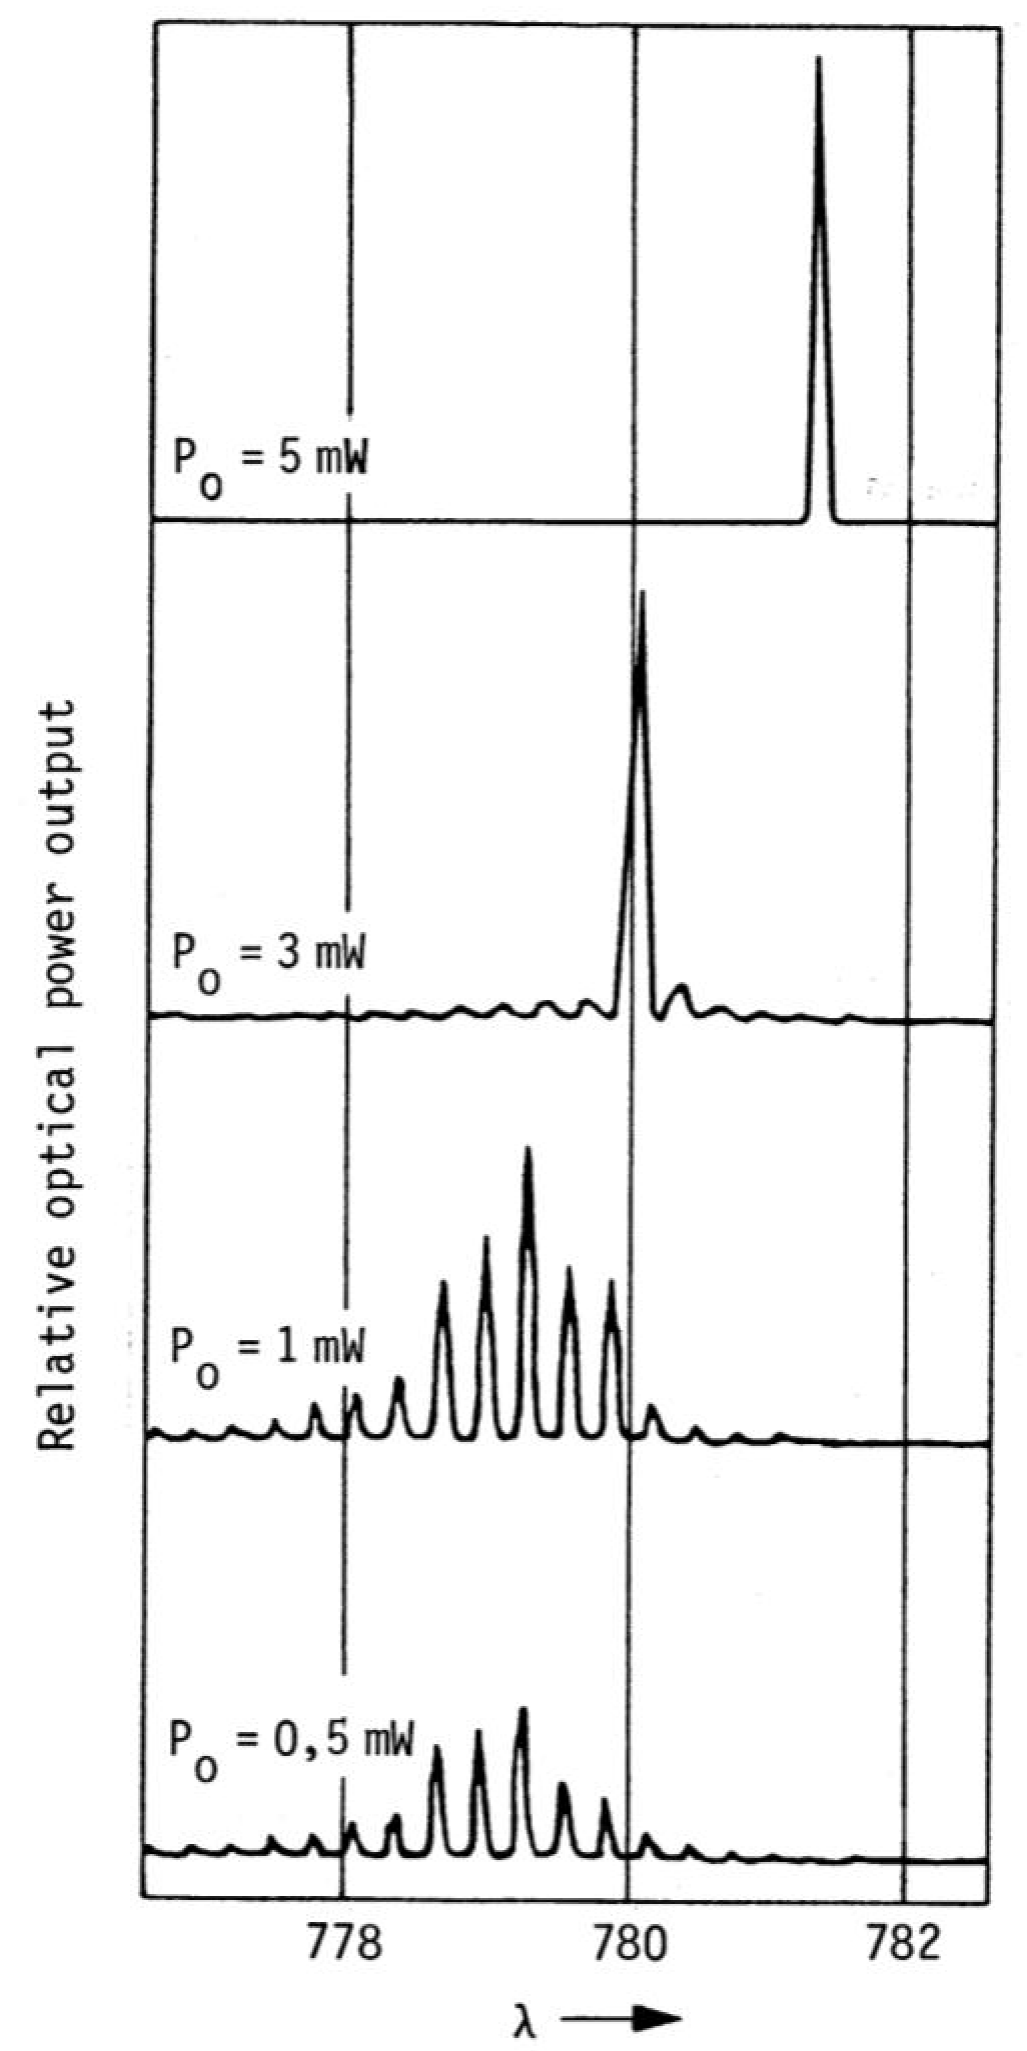
\includegraphics[width=.3\columnwidth]{Grafiken/Q1.png}%
\caption{output spectra of a laser diode for different optical output powers.}%
\label{fig:Q1}%
\end{figure}
The output spectra of a laser diode is shown in figure \ref{fig:Q1}\footnote[1]{Optical Communications Lab - Experiment 1, Preparation Materials} for different output powers $P_0$. 
There are different modes in the output spectrum.  How much modes exist depends on the optical gain each mode experiences. For a low output power the the spectrum is multimoded, for a higher power it gets single mode.\footnote[2]{Optoelectronics and Photonics; S. O. Kasap; Prentice Hall, 2001}
For higher powers the spectrum of the laser shifts to a longer wavelength.
An applied current through the flows nearly complete through the active zone of the laser diode. Because the refractive index depends on the carrier density\footnote[3]{Optische Nachrichtentechnik; Grau, G.; Freunde, W.; 3. ed.; Springer 1991} it changes with higher currents and therefore with higher optical output powers.

Since the resonance frequencies of the laser depend on the refractive index of the material, the frequencies shift with the higher output power as well.

\todo{nochmal kontrollieren, und warum �ndert sich der optical gain auch mit der leistung? sicher auch wegen $\Delta n$.}